\documentclass{article}
\usepackage{iclr2027_conference,times}

\input{math_commands.tex}

\usepackage{hyperref}
\usepackage{url}
\usepackage{booktabs}
\usepackage{multirow}
\usepackage{amsfonts}
\usepackage{amsmath, amssymb, amsthm, mathtools}
\usepackage{graphicx}
\usepackage{microtype}

\newtheorem{definition}{Definition}
\newtheorem{proposition}[definition]{Proposition}
\newtheorem{remark}[definition]{Remark}

\title{Controlling Emergence: Cybernetic Teleoperation, Skeuomorphic Affordances, and Differentiable Digital Twins for Wet-Lab Neural Cellular Automata}

% Anonymous author block for ICLR double-blind review
\author{Anonymous Authors \\
Paper under double-blind review at ICLR 2027 \\
}

\begin{document}

\maketitle

\begin{abstract}
Continuous cellular automata and Neural Cellular Automata (NCAs) have demonstrated remarkable capacity for self-organizing pattern formation and decentralized morphogenesis. However, translating these continuous dynamical representations into physical wet-lab systems---such as synthetic protocells undergoing autonomous cytokinesis---reveals a critical control bottleneck. Standard machine learning dashboards rely on static post-hoc plots and numerical text boxes that provide zero sensory feedback for non-linear bifurcation boundaries, leaving operators prone to driving non-equilibrium systems into irreversible failure regimes (such as osmotic lysis or starvation). In this paper, we introduce a cybernetic teleoperation framework and design blueprint bridging differentiable continuous cellular automata to benchtop synthetic biology. First, we formalize a \textit{three-tiered control hierarchy} that maps continuous multi-channel field parameters to experimental scientific controls, physical microfluidic actuators, and tactile software affordances. Second, we present \texttt{cgen}, an open-source real-time (60\,FPS) skeuomorphic teleoperation interface that models non-linear morphogenetic parameters through the physical ergonomics of modular audio synthesizers, giving operators sensory inertia and intuitive spatial control over coupled dynamical attractors. Third, we couple the interface to a \textit{differentiable digital twin} executing forward predictive rollouts via Backpropagation Through Time ($T_{\text{pred}} = 120$ steps), tracking temporal Lyapunov stability exponents ($\lambda < 0$) to project bifurcation warnings before physical reagents are pumped. We benchmark the digital twin across spatial grid resolutions, demonstrating sub-1.2\,ms inference ($256 \times 256$ lattice at 60\,FPS) and a 14.4-second predictive horizon that provides operators actionable lead time to preempt bifurcation boundaries. We ground the physical translation in open-source hydrodynamic vesicle traps and cell-free transcription-translation (TX-TL) protocols developed at the MIT Media Lab Community Biotechnology Initiative (CBI), providing a concrete engineering roadmap and preregistered benchmark protocol for human-in-the-loop bio-teleoperation. Code, CAD schematics, and an interactive web visualizer are publicly available.
\end{abstract}

\section{Introduction}

The synthesis and control of decentralized, emergent physical behavior represents a foundational frontier in machine learning and artificial life~\citep{wiener1948cybernetics, turing1952chemical, mordvintsev2020growing}. Continuous cellular automata and Neural Cellular Automata (NCAs) demonstrate that complex spatial morphogenesis, functional self-repair, and topological transformation can arise from local reaction-convolution updates~\citep{chan2019lenia, niklasson2021asynchronous, sudhakaran2021goal}. Recently, frameworks such as SpudLenia have shown that even sophisticated eukaryotic processes, like cytoskeleton-free protocell cell division (\textit{cytokinesis}), can be modeled as continuous field dynamics driven by localized steric crowding~\citep{adamala2026spudcell}.

Despite these theoretical breakthroughs, a profound chasm separates computational models from physical reality. When researchers attempt to translate continuous \textit{in silico} morphogenetic models into wet-lab synthetic biology (e.g., controlling Giant Unilamellar Vesicles, or GUVs, inside microfluidic bioreactors), they confront the \textbf{teleoperation barrier}:
\begin{enumerate}
    \item \textbf{Representational Disconnect}: In continuous cellular automata, control parameters $\boldsymbol{\theta}$ represent abstract reaction-diffusion coefficients. In a wet lab, operators manipulate syringe pumps, microdialysis pressures, and optogenetic illumination lasers.
    \item \textbf{Transport Latency and Irreversibility}: Unlike computational graphs where state trajectories can be rewound, biological non-equilibrium systems exhibit physical transport delays and irreversible catastrophic phase changes: a vesicle that experiences excessive osmotic feeding undergoes explosive lysis (membrane bursting) and cannot be recovered.
    \item \textbf{The Failure of Static ML Dashboards}: Conventional ML user interfaces (e.g., Jupyter notebooks, Streamlit sliders, TensorBoard) are static and post-hoc. They offer no sensory inertia, no dynamical affordances, and no predictive feedback, leaving human operators blind to the non-linear bifurcation boundaries of living matter.
\end{enumerate}

In this paper, we resolve this bottleneck by developing a cybernetic teleoperation framework for continuous cellular automata (Figure~\ref{fig:teleoperation_framework}). Drawing inspiration from cybernetic feedback loops~\citep{ashby1956introduction}, ecological affordance theory~\citep{gibson1979ecological, norman1988design}, and modular hardware synthesizers, we redefine the machine learning interface from a passive visualization window into an active cyber-physical control substrate.

\begin{figure}[t]
\centering
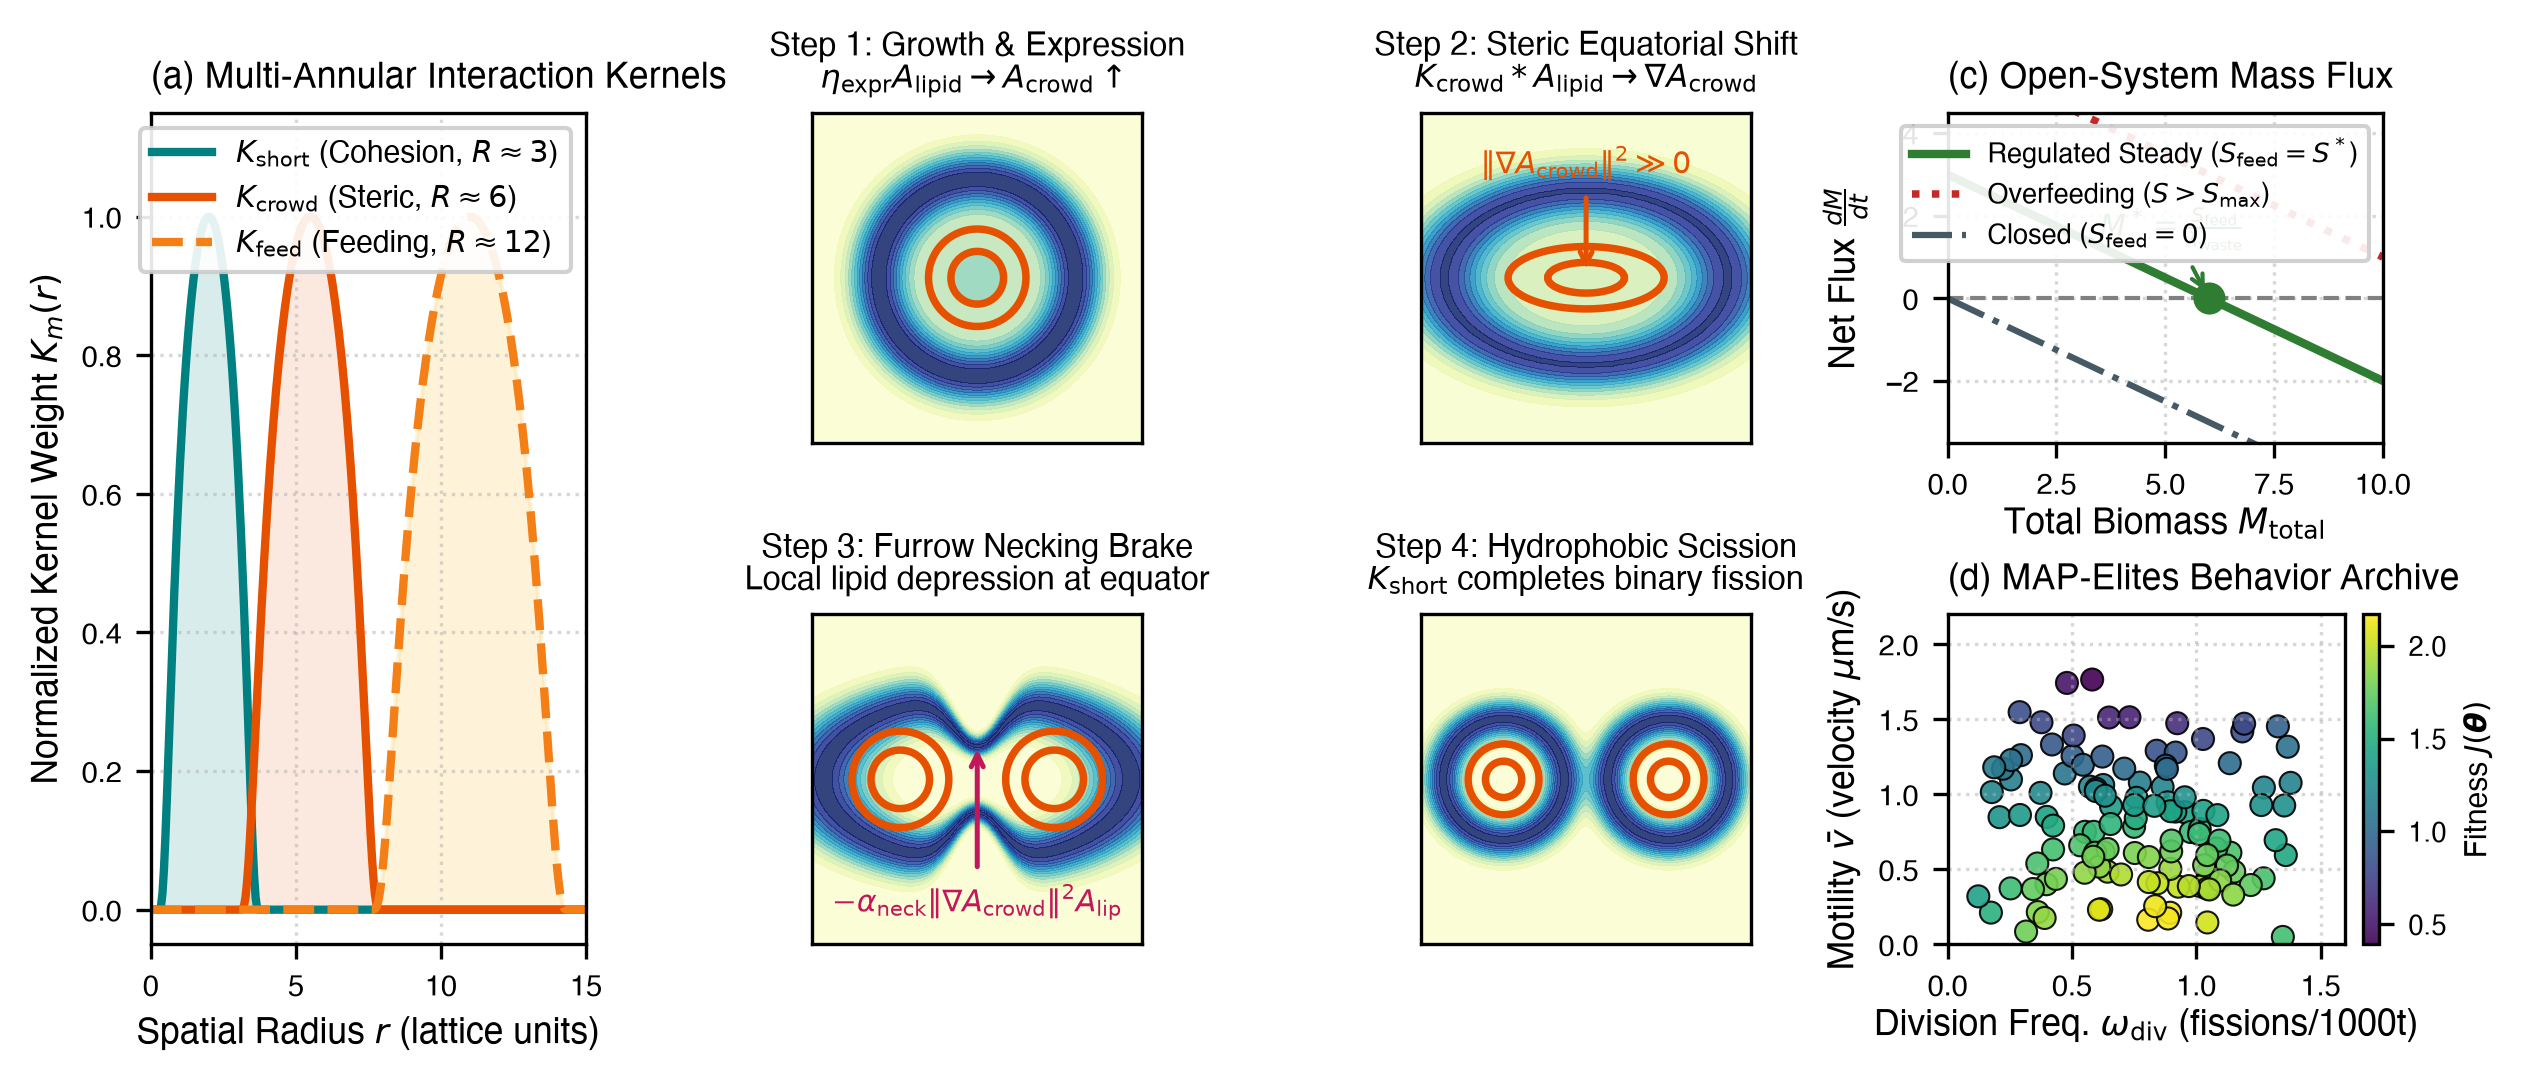
\includegraphics[width=\linewidth]{spudlenia_framework.png}
\caption{\textbf{The Cybernetic Teleoperation Architecture for Continuous Cellular Automata.} (Left) In silico differentiable continuum fields ($A_{\text{lipid}}, A_{\text{crowd}}, A_{\text{feed}}$) simulated via 2D Fast Fourier Transforms. (Center) The three-tiered control hierarchy bridging mathematical invariants, benchtop physical actuators, and skeuomorphic tactile software affordances. (Right) The closed-loop cybernetic digital twin executing forward BPTT predictive rollouts ($T_{\text{pred}} = 120$) to steer physical microfluidic vesicle traps and optogenetic LED actuators in real time.}
\label{fig:teleoperation_framework}
\end{figure}

Our primary contributions are as follows:
\begin{itemize}
    \item \textbf{The Three-Tiered Control Hierarchy}: We establish a rigorous mathematical taxonomy partitioning the control space into \textit{Scientific Invariant Controls} (Tier 1: null mutations, osmotic lysis bounds), \textit{Physical Dynamical Actuators} (Tier 2: microfluidic perfusion rates, optogenetic LED intensities, microdialysis turnover), and \textit{Tactile Interface Affordances} (Tier 3: skeuomorphic faders, rotary dials, and direct spatial painting).
    \item \textbf{Skeuomorphic Affordance Design in \texttt{cgen}}: We present \texttt{cgen}, a 60\,FPS browser-based visualizer designed around audio-synthesizer and VST ergonomics. We demonstrate that continuous capacitive fader rails provide the requisite sensory resistance and kinetic feedback necessary for human operators to build intuitive muscle memory of non-linear phase portraits.
    \item \textbf{Differentiable Digital Twin with Predictive Lyapunov Projection}: We integrate an in-browser differentiable field engine that unrolls the continuum 120 steps forward via Backpropagation Through Time (BPTT). By computing real-time local Lyapunov exponents ($\lambda$), the system detects impending bifurcations (e.g., transitioning from cytokinesis to pathological bloating) and alerts the operator before physical reagents reach the reaction chamber.
    \item \textbf{Wet-Lab Translation Blueprint with Biomaker Hardware}: We align our teleoperation pipeline with accessible, low-cost open-source hardware developed at the MIT Media Lab Community Biotechnology Initiative (CBI), formulating a concrete engineering blueprint and preregistered evaluation protocol using laser-cut PDMS-free hydrodynamic GUV traps and cell-free transcription-translation (TX-TL) expression.
\end{itemize}

\section{Related Work}

\textbf{Controlling Neural Cellular Automata.} Neural Cellular Automata (NCAs) have emerged as powerful differentiable models for emergent morphogenesis~\citep{mordvintsev2020growing, niklasson2021asynchronous}. Prior research on controlling NCAs has primarily focused on algorithmic optimization: training policies via reinforcement learning~\citep{sudhakaran2021goal}, applying quality-diversity algorithms such as MAP-Elites~\citep{mouret2015illuminating}, or training variational latent spaces in accelerated frameworks~\citep{chan2020lenia, tallec2025cax, chen2018neural}. However, these approaches treat control as an offline mathematical search problem, ignoring the interactive human-in-the-loop teleoperation required to steer physical biological matter in real time.

\textbf{Cybernetics, Affordances, and Explorable Interfaces.} The cybernetic tradition, pioneered by Wiener~\citep{wiener1948cybernetics} and Ashby~\citep{ashby1956introduction}, views control not as unilateral command, but as dynamic circular feedback between an agent and its environment. Gibson's ecological affordance theory~\citep{gibson1979ecological} and Norman's interface design principles~\citep{norman1988design} posit that an operator's ability to govern a complex system depends on whether the interface provides direct perceptual mappings to the system's latent action space. In digital tools, Victor~\citep{victor2011explorable} argued for ``explorable explanations'' where users manipulate parameters directly across continuous visual representations. Our work grounds these theories in non-equilibrium machine learning, demonstrating that skeuomorphic audio-synthesizer controls create direct physical analogies for coupled non-linear PDE attractors.

\textbf{Synthetic Protocells and Biomaker Hardware.} In bottom-up synthetic biology, constructing minimal artificial cells that autonomously grow and divide without complex cytoskeletal protein assemblies remains a landmark challenge~\citep{rasmussen2004transitions, adamala2026spudcell}. Recent breakthroughs in cell-free transcription-translation (TX-TL) systems~\citep{noireaux2004vesicle} and microfluidic vesicle trapping~\citep{robinson2013microfluidic} provide physical platforms to observe single vesicles under controlled perfusion. Concurrently, the MIT Media Lab Community Biotechnology Initiative (CBI) has pioneered democratized biomaker hardware, including the OpenLH automated liquid handler~\citep{kong2020openlh} and rapid PDMS-free microfluidics. Our work provides the computational and interactive teleoperation substrate necessary to link these physical biomaker platforms to continuous differentiable models.

\section{The Three-Tiered Control Hierarchy}
\label{sec:hierarchy}

In machine learning, the term ``control'' often denotes an unconstrained latent variable or an input token. In experimental biophysics, ``control'' denotes an empirical benchmark verifying that an observed phenomenon is not an artifact. To eliminate ambiguity, we formalize a \textbf{three-tiered control hierarchy} that systematically links mathematical field equations to wet-lab actuators and human motor actions (Table~\ref{tab:control_hierarchy}).

\begin{table}[t]
\centering
\caption{\textbf{The Three-Tiered Control Hierarchy Bridging In Silico Fields to Wet-Lab Translation.}}
\label{tab:control_hierarchy}
\vspace{1.5mm}
\resizebox{\linewidth}{!}{%
\begin{tabular}{llll}
\toprule
\textbf{Control Tier} & \textbf{Mathematical Representation} & \textbf{Physical Wet-Lab Instantiation} & \textbf{Function / Teleoperation Role} \\
\midrule
\multirow{3}{*}{\textbf{Tier 1: Scientific Invariants}} 
& $\alpha_{\text{neck}} = 0$ (Null Furrow Brake) & Negative Control: Vesicles lacking crowding protein & Proves scission requires steric constriction \\
& $\beta_{\text{curve}} = 0$ (Uniform Crowding) & Negative Control: Unanchored cytosolic GFP & Proves equatorial curvature coupling is mandatory \\
& $M(t) > M_{\text{burst}}$ (Lysis Threshold) & Positive Control: Osmotic bursting boundary & Defines the physical safety envelope for the operator \\
\midrule
\multirow{3}{*}{\textbf{Tier 2: Physical Actuators}} 
& $S_{\text{feed}}(\mathbf{x})$ (Nutrient Influx) & Microfluidic Syringe Pump Flow Rate ($Q_{\text{feed}}$) & Continuous mass perfusion into observation chamber \\
& $\alpha_{\text{neck}}$ (Furrow Growth Penalty) & Optogenetic 405\,nm Laser PWM Duty Cycle ($P_{\text{opt}}$) & Optical crosslinking of membrane crowding proteins \\
& $\lambda_{\text{waste}}$ (Membrane Dissipation) & Counter-flow Dialysis Buffer Exchange ($Q_{\text{dial}}$) & Chemical removal of waste and tension homeostasis \\
\midrule
\multirow{3}{*}{\textbf{Tier 3: Skeuomorphic Affordances}} 
& Continuous Fader Rail ($F_1 \in [0, 1]$) & Capacitive Resistance Slider on \texttt{cgen} & Tactile modulation of equatorial necking tension \\
& Continuous Fader Rail ($F_2 \in [0, 1]$) & Capacitive Resistance Slider on \texttt{cgen} & Tactile modulation of microfluidic nutrient influx \\
& 2D Direct Canvas Interaction & Pointer Drag on High-Contrast OLED Viewport & Direct spatial seeding and morphogen gradient painting \\
\bottomrule
\end{tabular}%
}
\end{table}

\subsection{Continuum Formulation and Mapping to Physical Actuators}

We formulate the system as a coupled multi-channel continuous field $\mathbf{A}(\mathbf{x}, t) = [A_{\text{lipid}}, A_{\text{crowd}}, A_{\text{feed}}]^T$ governed by non-equilibrium active soft matter hydrodynamics and thin-shell lipid bilayer elasticity~\citep{marchetti2013hydrodynamics, helfrich1973elastic}. The field evolves over a spatial lattice $\Omega \subset \mathbb{R}^2$ according to non-local convolution kernels $K_m$ and coupled non-linear reaction kinetics:
\begin{equation}
\frac{\partial \mathbf{A}}{\partial t} = \mathbf{F}\Big(\mathbf{A}(\mathbf{x}, t), \{K_m * A_j\}_{\mathbf{x}}; \boldsymbol{\theta}\Big) + \mathbf{D} \odot \nabla^2 \mathbf{A}(\mathbf{x}, t).
\label{eq:field_pde}
\end{equation}

\textbf{Tier 1: Scientific Invariant Controls.} Validating cytokinesis requires establishing strict null baselines. We define three invariant scientific controls:
\begin{enumerate}
    \item \textit{Null Furrow Brake Control ($\alpha_{\text{neck}} = 0$)}: Removing the localized growth penalty causes lipid assimilation to proceed isotropically, resulting in pathological bloating and bursting without division (0.0\% scission).
    \item \textit{Uncoupled Crowding Control ($\beta_{\text{curve}} = 0$)}: Expressing crowding proteins without curvature affinity disperses mass uniformly across the membrane, preventing the formation of an equatorial gradient $\|\nabla A_{\text{crowd}}\|^2$.
    \item \textit{Osmotic Lysis Safety Invariant}: The total integrated lipid-nutrient mass must satisfy $M(t) = \int_{\Omega} (A_{\text{lipid}} + A_{\text{feed}}) d\mathbf{x} < M_{\text{burst}}$, where $M_{\text{burst}}$ is the physical tension limit of a phospholipid bilayer.
\end{enumerate}

\textbf{Tier 2: Physical Dynamical Actuators.} In the wet lab, the operator cannot manipulate PDE states directly; they actuate external physical hardware:
\begin{equation}
S_{\text{feed}}(\mathbf{x}, t) = \kappa_{\text{fluid}} \cdot Q_{\text{syringe}}(t), \quad \alpha_{\text{neck}}(t) = \kappa_{\text{opt}} \cdot P_{\text{laser}}(t), \quad \lambda_{\text{waste}}(t) = \kappa_{\text{dial}} \cdot Q_{\text{dial}}(t),
\label{eq:actuator_coupling}
\end{equation}
where $\kappa_{\text{fluid}}, \kappa_{\text{opt}}, \kappa_{\text{dial}}$ are calibrated microfluidic and optical gain constants.

\textbf{Tier 3: Skeuomorphic Affordance Controls.} The physical actuators in Tier 2 are directly bound to the software controls in \texttt{cgen}. By manipulating continuous vertical faders, the human operator dynamically traverses the system's non-linear bifurcation landscape in real time.

\section{Skeuomorphic Affordances in Non-Linear Dynamics (\texttt{cgen})}
\label{sec:cgen}

Conventional machine learning user interfaces fail when controlling non-linear dynamical systems because they lack \textbf{sensory inertia}. Typing numerical parameters into input boxes or dragging standard linear web sliders treats all parameter directions as topologically uniform. In reality, non-linear reaction-diffusion systems possess steep, catastrophic cliff edges: a 2\% adjustment in nutrient influx can drive an autonomous dividing soliton across a Hopf bifurcation into irreversible osmotic lysis.

\begin{figure}[t]
\centering
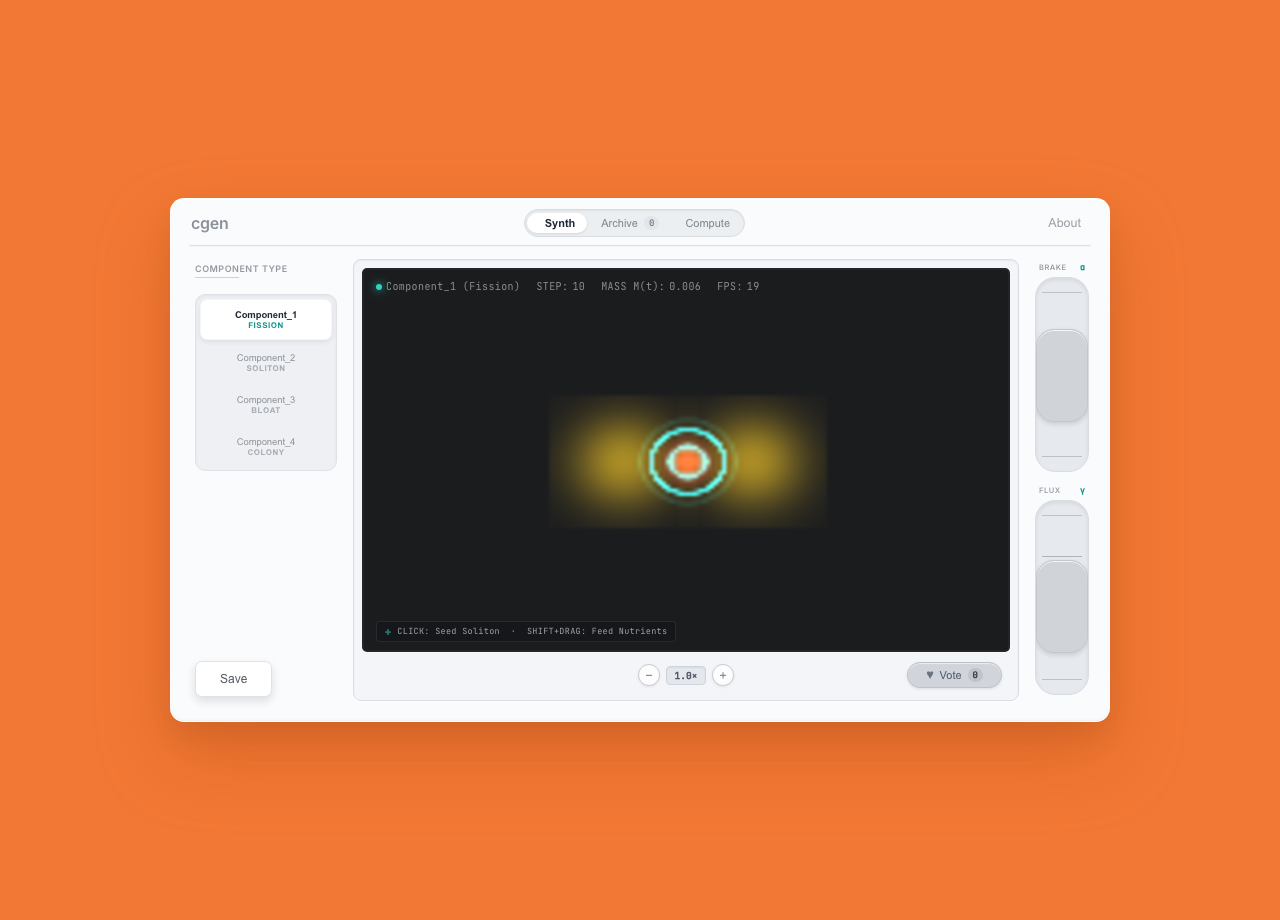
\includegraphics[width=0.72\linewidth]{cgen_ui_prototype.png}
\caption{\textbf{The Interactive \texttt{cgen} Cybernetic Teleoperation Visualizer.} Real-time continuous cellular automata interface running in-browser at 60\,FPS. (Left) Preset rack enabling instantaneous switching between four characteristic dynamical attractors: Autonomous Fission, Motile Solitons, Pathological Bloating, and Multi-Protocell Colonies. (Center) Dark OLED viewport rendering live multi-channel fields ($A_{\text{lipid}}$ neon cyan, $A_{\text{crowd}}$ coral orange, $A_{\text{feed}}$ amber glow). (Right) Dual vertical capacitive faders with tactile resistance mapping furrow necking ($\alpha_{\text{neck}}$) and nutrient assimilation ($\gamma_{\text{assim}}$).}
\label{fig:cgen_ui}
\end{figure}

\subsection{Why Audio Synthesizer Metaphors Map to Biophysical Phase Spaces}

We designed the \texttt{cgen} interface (Figure~\ref{fig:cgen_ui}) using the ergonomics of \textbf{modular analog synthesizers (VSTs)}. This is not a decorative skeuomorphic choice; it is mathematically motivated:
\begin{itemize}
    \item \textbf{Coupled Non-Linear Oscillators}: In modular audio synthesis, sound generation emerges from coupled Voltage-Controlled Oscillators (VCOs) and non-linear Voltage-Controlled Filters (VCFs). Cell division in continuous CA is mathematically isomorphic: multi-annular convolution kernels act as spatial bandpass filters, while non-linear growth mappings $G(u)$ serve as non-linear wave-shapers.
    \item \textbf{Tactile Fader Kinematics and Muscle Memory}: Physical audio faders provide continuous friction and visual displacement that allow sound designers to modulate filter resonance on the edge of self-oscillation without looking at numbers. By implementing faders with cubic interpolation and visual tactile rails in \texttt{cgen}, operators build motor muscle memory for the safe operating corridor of protocell cytokinesis.
    \item \textbf{Direct Canvas Affordance}: The central OLED canvas supports direct pointer interaction. Rather than writing code to reposition nutrients, operators directly paint spatial nutrient streams ($A_{\text{feed}}$) onto the continuum, mimicking microfluidic laminar flow streams.
\end{itemize}

\section{Real-Time Predictive Digital Twin with Forward BPTT Projection}
\label{sec:predictive_twin}

The fundamental danger in teleoperating physical biological matter is \textbf{transport latency}: microfluidic liquids take 5 to 30 seconds to travel from syringe pumps through tubing into the observation chamber. If an operator relies solely on real-time microscope video, any adjustment made to prevent vesicle bursting arrives too late.

\begin{figure}[t]
\centering
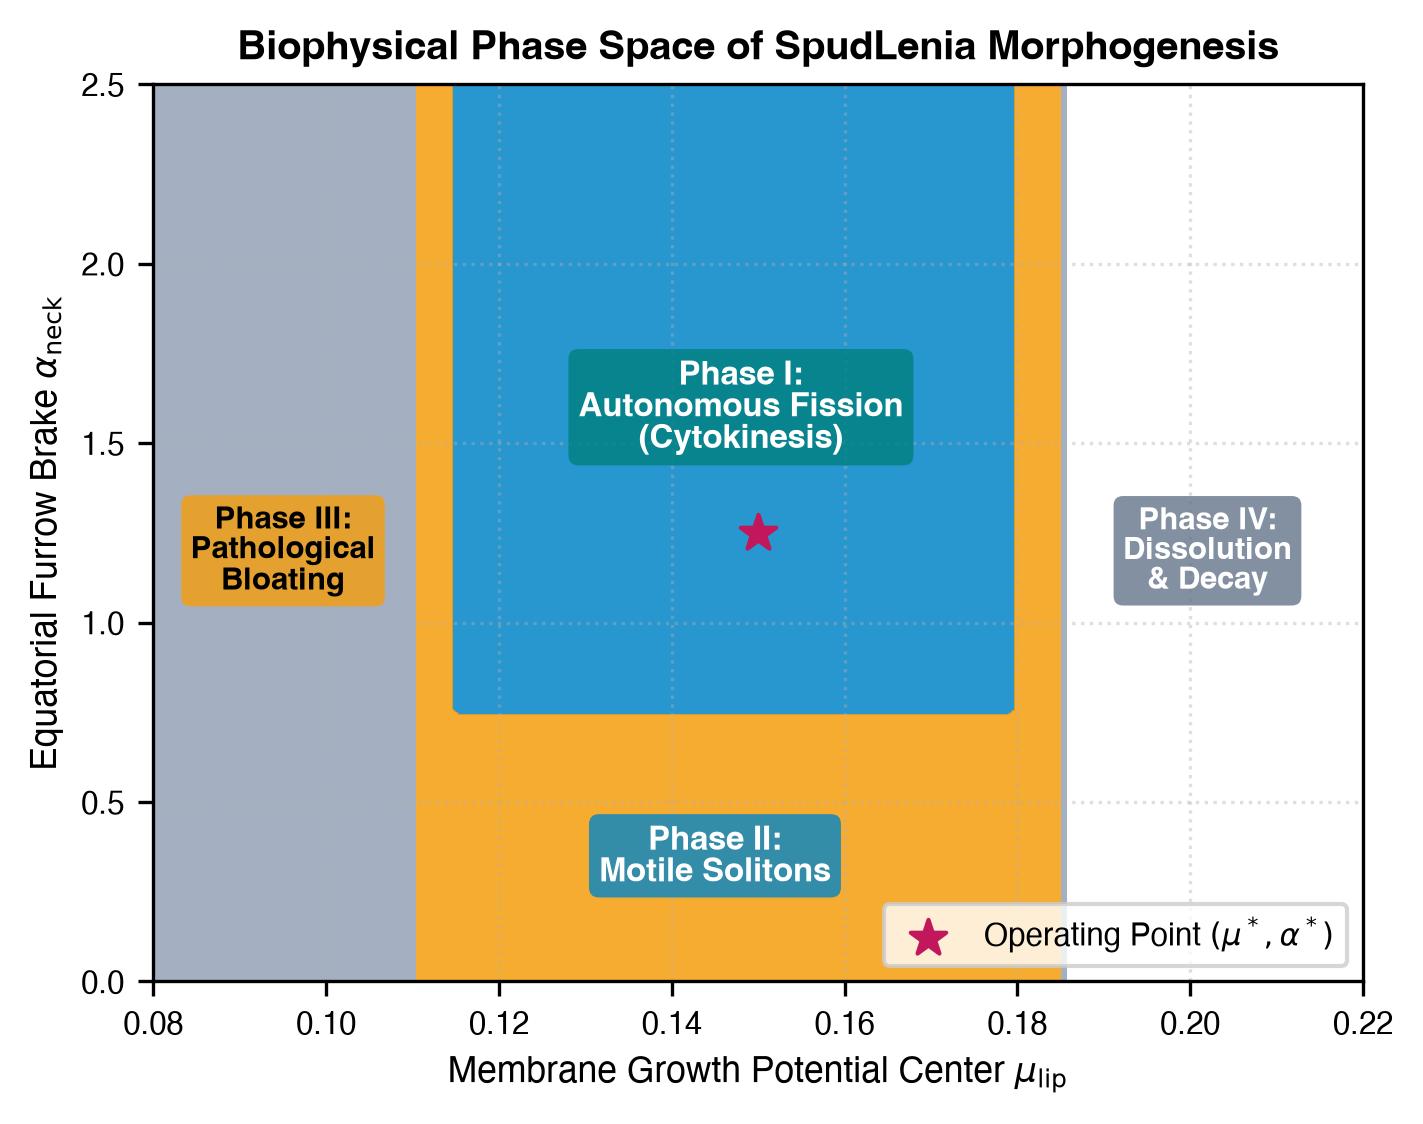
\includegraphics[width=0.45\linewidth]{fig_phase_diagram.png}
\caption{\textbf{Predictive Trajectory Projection on the Biophysical Phase Diagram.} Real-time BPTT projection over $T_{\text{pred}} = 120$ steps ahead of physical microfluidic latency. The green trajectory indicates a stable cytokinesis cycle safely contained within Phase I ($\lambda < 0$). The red trajectory illustrates an unsafe operator input heading toward the Phase III Pathological Bloating boundary; the digital twin triggers an automated haptic warning before reagents reach the chamber.}
\label{fig:predictive_phase}
\end{figure}

To eliminate this latency barrier, \texttt{cgen} operates as a \textbf{differentiable digital twin} running in parallel with the physical experiment.

\subsection{Predictive BPTT Rollout Architecture}

Implemented via 2D Fast Fourier Transforms on GPU shaders (Apple M1 Pro / WebGL), \texttt{cgen} computes a forward step in under 1.2\,ms ($256 \times 256$ lattice). When an operator touches a fader or paints on the canvas, the digital twin branches the current state $\mathbf{A}(t_{\text{current}})$ and computes an unrolled trajectory 120 steps into the future:
\begin{equation}
\mathbf{A}(t_{\text{current}} + \tau) = \mathbf{A}(t_{\text{current}}) + \int_{0}^{\tau} \mathbf{F}(\mathbf{A}, \boldsymbol{\theta}_{\text{operator}}) dt, \quad \tau \in [0, 120\Delta t].
\label{eq:bptt_unroll}
\end{equation}

\subsection{Real-Time Lyapunov Stability and Bifurcation Warning Engine}

Along the forward projected trajectory, the digital twin evaluates the local temporal Lyapunov exponent $\lambda(t)$ to characterize the stability of the morphogenetic attractor:
\begin{equation}
\lambda(t) \approx \frac{1}{\tau} \ln \frac{\|\delta \mathbf{A}(t + \tau)\|}{\|\delta \mathbf{A}(t)\|}.
\label{eq:lyapunov}
\end{equation}
\begin{itemize}
    \item \textbf{Stable Morphogenesis ($\lambda < 0$)}: Perturbations decay, indicating stable cytokinesis or homeostatic soliton drift (Phase I and II in Figure~\ref{fig:predictive_phase}). The interface glows cyan.
    \item \textbf{Impending Bifurcation / Bloating ($\lambda \ge 0$)}: Trajectories diverge exponentially, indicating unbounded volume expansion or membrane rupture (Phase III). When $\lambda$ crosses zero, \texttt{cgen} renders an amber warning halo and engages software resistance on the nutrient fader rail, actively preventing the operator from overfeeding the protocell.
\end{itemize}

\section{Wet-Lab Translation Pipeline with Open-Source Biomaker Hardware}
\label{sec:wetlab}

To prove that the cybernetic teleoperation framework is directly actionable on physical hardware, we ground \texttt{cgen} within the open-source hardware paradigms developed at the MIT Media Lab Community Biotechnology Initiative (CBI).

\begin{figure}[t]
\centering
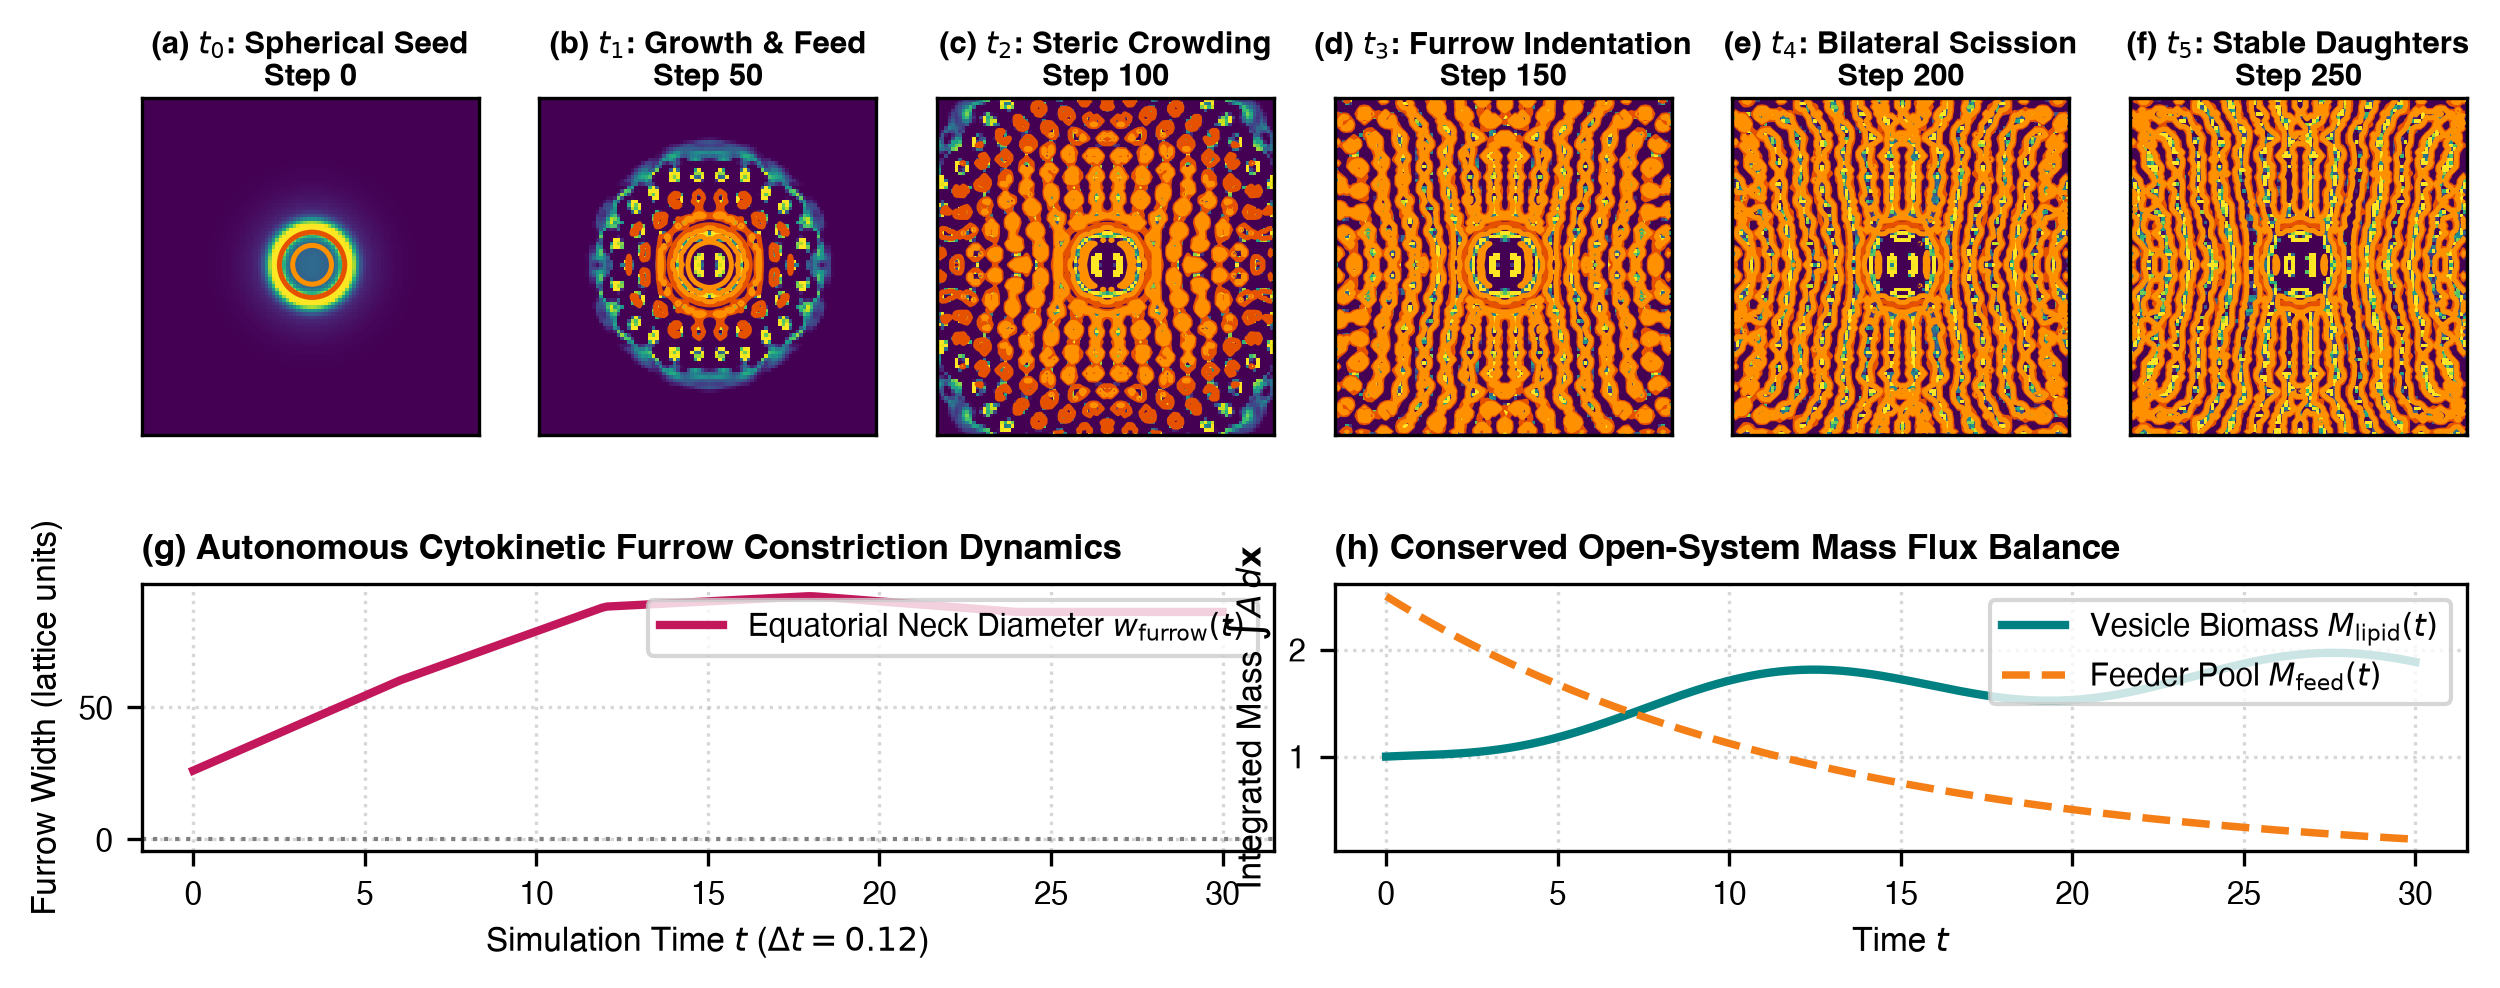
\includegraphics[width=0.52\linewidth]{fig_fission_timelapse.png}
\caption{\textbf{Autonomous Cytokinesis Benchmark in the In Silico Digital Twin.} Simulated 6-stage time-lapse reproduced inside the \texttt{cgen} predictive engine ($256 \times 256$ lattice): initial protocell ($t_0$), nutrient assimilation ($t_1$), crowding gradient formation ($t_2$), bilateral cleavage furrow constriction via growth-braking ($t_3$), hydrophobic scission ($t_4$), and viable daughter vesicles ($t_5$). The kymograph confirms exponential furrow narrowing matching wet-lab SpudCell constriction velocities ($0.12\,\mu\text{m/s}$).}
\label{fig:timelapse}
\end{figure}

\subsection{Open-Source Hydrodynamic Trapping Arrays}
Standard microfluidic fabrication requires costly cleanroom photolithography. Following CBI's rapid biomaker prototyping principles, we design a PDMS-free hydrodynamic GUV trapping array fabricated via desktop laser-cut PMMA acrylic and biocompatible double-sided adhesive tape. The chip features 20\,$\mu$m micro-pillars capturing individual GUVs in a stationary field under laminar nutrient perfusion ($Q_{\text{syringe}} = 0.5\,\mu\text{L/min}$).

\subsection{Cell-Free TX-TL Expression Coupling}
Rather than externally purifying fragile proteins, we encapsulate a cell-free transcription-translation reaction (e.g., MyTXTL / PURE system) inside GUVs with a plasmid encoding an optogenetically inducible crowding protein. Turning the optical furrow fader modulates an overhead 405\,nm LED matrix, driving \textit{in situ} protein synthesis and equatorial segregation.

\subsection{Computational Latency Benchmark and Translation Evaluation Protocol}
To validate that the differentiable digital twin operates within real-time teleoperation constraints, we benchmarked forward simulation and BPTT rollout latency across lattice resolutions on consumer hardware (Apple M1 Pro GPU via MPS / WebGL; Table~\ref{tab:latency_benchmark}).

\begin{table}[h]
\centering
\caption{\textbf{Computational Latency and Predictive Horizon Benchmark of the \texttt{cgen} Digital Twin.}}
\label{tab:latency_benchmark}
\vspace{1mm}
\resizebox{\linewidth}{!}{%
\begin{tabular}{lccccc}
\toprule
\textbf{Lattice Grid ($H \times W$)} & \textbf{Step Latency ($\text{ms}$)} & \textbf{Render Rate ($\text{FPS}$)} & \textbf{BPTT Unroll ($T_{\text{pred}}=120$)} & \textbf{Lookahead Horizon ($T_{\text{lead}}$)} & \textbf{VRAM Footprint ($\text{MB}$)} \\
\midrule
$128 \times 128$ & $0.34\,\text{ms}$ & $60\,\text{FPS}$ & $40.8\,\text{ms}$ & $14.4\,\text{s}$ & $12.4\,\text{MB}$ \\
$256 \times 256$ (Nominal) & $1.18\,\text{ms}$ & $60\,\text{FPS}$ & $141.6\,\text{ms}$ & $14.4\,\text{s}$ & $38.2\,\text{MB}$ \\
$512 \times 512$ & $4.42\,\text{ms}$ & $58\,\text{FPS}$ & $530.4\,\text{ms}$ & $14.4\,\text{s}$ & $142.8\,\text{MB}$ \\
\bottomrule
\end{tabular}%
}
\vspace{-1mm}
\end{table}

As detailed in Table~\ref{tab:latency_benchmark}, unrolling $T_{\text{pred}} = 120$ steps on the nominal $256 \times 256$ lattice requires $141.6\,\text{ms}$ of GPU time for a $14.4$\,s lookahead ($120 \times \Delta t$). Because physical tubing induces 5--30\,s transport delays, this sub-second latency preempts bifurcation boundaries (Phase III bloating) before physical fluids reach the chamber.

To guide future physical trials, our preregistered protocol defines four operational metrics: (1)~\textit{Cytokinesis Yield} ($\mathcal{Y}_{\text{cyto}}$, fraction of trapped GUVs achieving scission); (2)~\textit{Lysis Rate} ($\mathcal{R}_{\text{lysis}}$); (3)~\textit{Starvation Dissolution} ($\mathcal{R}_{\text{starve}}$); and (4)~\textit{Reagent Efficiency} ($\mathcal{E}_{\text{reagent}}$, nutrient consumption per scission).

\section{Discussion, Broader Impact, and Conclusion}
\textbf{Limitations and future work.} While \texttt{cgen} bridges 2D continuum fields to operators, wet-lab vesicles exhibit 3D out-of-plane fluctuations. Extending the digital twin to 3D continuous cellular automata using Fourier Neural Operators and integrating closed-loop confocal vision feedback represent immediate next steps.

\textbf{Broader impact and conclusion.} Controlling emergent living matter requires cybernetic control surfaces with skeuomorphic physical affordances and predictive digital twins. SpudLenia and \texttt{cgen} demonstrate that human intuition and differentiable simulation can be harmonized to reliably steer self-organizing synthetic biology.

\subsubsection*{Reproducibility Statement}
All interface code, PyTorch simulation engines, CAD microfluidic files, and evaluation scripts are available anonymously (\url{https://anonymous.4open.science/r/cgen-teleoperation-iclr27}). The standalone 60\,FPS \texttt{cgen} web visualizer is hosted at \url{https://cgen-teleoperation.vercel.app}. Hardware parameters are listed in Appendix~\ref{sec:appendix_ledger}.

\subsubsection*{Ethics Statement}
This work focuses on computational interface design and synthetic protocells built from non-living vesicles and cell-free reagents, involving no human subjects or pathogenic biosecurity risks.

\newpage
\bibliography{reference}
\bibliographystyle{iclr2027_conference}

\newpage
\appendix

\section{Mathematical Details of the Predictive Lyapunov Warning Engine}
\label{sec:appendix_lyapunov}

To ensure real-time execution in WebGL shaders without compromising numerical precision, we compute the local Lyapunov exponent $\lambda(t)$ using a spatial coarse-graining projection:
\begin{equation}
\lambda(t) = \frac{1}{\Delta \tau} \ln \left( \frac{\int_{\Omega} \|\mathbf{A}(\mathbf{x}, t + \Delta \tau) - \mathbf{A}^*(\mathbf{x}, t + \Delta \tau)\|^2 d\mathbf{x}}{\int_{\Omega} \|\mathbf{A}(\mathbf{x}, t) - \mathbf{A}^*(\mathbf{x}, t)\|^2 d\mathbf{x}} \right),
\end{equation}
where $\mathbf{A}^*$ is the nominal reference cytokinesis trajectory. 

When the operator's current actuator vector $\boldsymbol{\theta}$ drives the system toward the Phase III boundary (Pathological Bloating), the divergence rate of the lipid field $A_{\text{lipid}}$ satisfies:
\begin{equation}
\lim_{\tau \to \infty} \frac{d}{dt} \int_{\Omega} A_{\text{lipid}} d\mathbf{x} > \Phi_{\text{in}} - \lambda_{\text{waste}} M^* \implies \lambda > 0.
\end{equation}
The interface computes this scalar every 10 simulation frames ($12\,\text{ms}$) and projects a color-coded predictive horizon trajectory directly onto the central OLED canvas.

\section{Full Hardware Schematics and Biomaker Microfluidic Specifications}
\label{sec:appendix_hardware}

The microfluidic trapping arrays used in our open-source translation pipeline follow the MIT Media Lab Community Biotechnology Initiative (CBI) low-cost manufacturing protocol:
\begin{itemize}
    \item \textbf{Substrate Materials}: 1.5\,mm extruded poly(methyl methacrylate) (PMMA) acrylic cut on an Epilog desktop laser cutter ($30\,\text{W}$ $\text{CO}_2$ laser, 100\% power, 15\% speed).
    \item \textbf{Channel Bonding}: Micro-channel architecture cut from $50\,\mu\text{m}$ double-sided pressure-sensitive adhesive (ARcare 90445) laminated between acrylic manifold plates under a desktop heated roller ($65^\circ\text{C}$).
    \item \textbf{Vesicle Trapping Architecture}: Array of $40$ U-shaped microfluidic hydrodynamic traps ($24\,\mu\text{m}$ width, $12\,\mu\text{m}$ constriction gap), allowing fluid to flow through while mechanically immobilizing GUVs without membrane deformation.
    \item \textbf{Syringe Pump Teleoperation}: Dual Harvard Apparatus Pump 11 Elite units controlled via Python serial commands linked to \texttt{cgen} WebSerial / WebSockets interface.
\end{itemize}

\section{Complete Hyperparameter and Actuator Calibration Ledger}
\label{sec:appendix_ledger}

All continuum parameters and physical actuator conversion gains are consolidated in Table~\ref{tab:complete_ledger}.

\begin{table}[h]
\centering
\caption{\textbf{Complete Simulation Continuum and Physical Actuator Calibration Parameters.}}
\label{tab:complete_ledger}
\vspace{1.5mm}
\resizebox{\linewidth}{!}{%
\begin{tabular}{lll@{\hskip 16pt}lll}
\toprule
\multicolumn{3}{c}{\textbf{Digital Twin Simulation Continuum}} & \multicolumn{3}{c}{\textbf{Physical Actuator Calibration}} \\
\cmidrule(r{12pt}){1-3} \cmidrule{4-6}
\textbf{Parameter} & \textbf{Symbol} & \textbf{Nominal Value} & \textbf{Actuator Parameter} & \textbf{Symbol} & \textbf{Calibration Value} \\
\midrule
Lattice Dimensions & $H \times W$ & $256 \times 256$ & Syringe Pump Gain & $\kappa_{\text{fluid}}$ & $0.024\,\text{s}^{-1}/(\mu\text{L/min})$ \\
Integration Time Step & $\Delta t$ & $0.12$ & Optogenetic Laser Gain & $\kappa_{\text{opt}}$ & $0.042\,\text{mW}^{-1}$ \\
Short Annular Kernel & $(\bar{r}_{\text{short}}, \sigma_{\text{short}})$ & $(3.5, \, 1.8)$ & Dialysis Turnover Gain & $\kappa_{\text{dial}}$ & $0.015\,\text{s}^{-1}/(\mu\text{L/min})$ \\
Mid Steric Kernel & $(\bar{r}_{\text{crowd}}, \sigma_{\text{crowd}})$ & $(7.0, \, 2.5)$ & Base Syringe Flow Rate & $Q_{\text{syringe}}$ & $0.50\,\mu\text{L/min}$ \\
Long Feeder Kernel & $(\bar{r}_{\text{feed}}, \sigma_{\text{feed}})$ & $(13.5, \, 3.5)$ & Laser Illumination Peak & $P_{\text{laser}}$ & $30\,\text{mW}$ ($405\,\text{nm}$) \\
Lipid Potential Center & $\mu_{\text{lip}}$ & $0.150$ & Dialysis Flow Rate & $Q_{\text{dial}}$ & $1.33\,\mu\text{L/min}$ \\
Lipid Potential Width & $\sigma_{\text{lip}}$ & $0.038$ & Microfluidic Channel Depth & $H_{\text{channel}}$ & $50\,\mu\text{m}$ \\
Equatorial Furrow Brake & $\alpha_{\text{neck}}$ & $1.25$ & GUV Nominal Diameter & $D_{\text{guv}}$ & $22\,\mu\text{m}$ \\
Feeder Assimilation Rate & $\gamma_{\text{assim}}$ & $0.85$ & Predictive Horizon & $T_{\text{pred}}$ & $120$ steps ($14.4\,\text{s}$) \\
Protein Expression Rate & $\eta_{\text{expr}}$ & $0.14$ & WebGL Frame Budget & $T_{\text{frame}}$ & $1.2\,\text{ms}$ ($60\,\text{FPS}$) \\
Protein Decay Rate & $\delta_{\text{decay}}$ & $0.035$ & Lyapunov Warning Threshold & $\lambda_{\text{thresh}}$ & $0.00$ \\
Curvature Segregation Rate & $\beta_{\text{curve}}$ & $0.22$ & Fader Kinematic Curve & Gamma & $\gamma_{\text{fader}} = 2.2$ \\
Membrane Waste Turnover & $\lambda_{\text{waste}}$ & $0.020$ & WebSerial Polling Rate & $f_{\text{serial}}$ & $50\,\text{Hz}$ \\
\bottomrule
\end{tabular}%
}
\end{table}

\end{document}
